\subsection{ Parte estrutural do sistema}

 O material escolhido para a estrutura foi o compensado, as chapas de compensado são materiais versáteis e amplamente utilizados na indústria da construção, marcenaria e artesanato. Elas são fabricadas a partir de finas lâminas de madeira, conhecidas como lâminas de folheado, coladas umas sobre as outras com fibras perpendiculares, conferindo maior estabilidade e resistência mecânica ao produto final, Figura \ref{fig3:image_02}.


\begin{figure}[!h]
	\centering
	\caption{Chapas de compensado.}
	\efbox{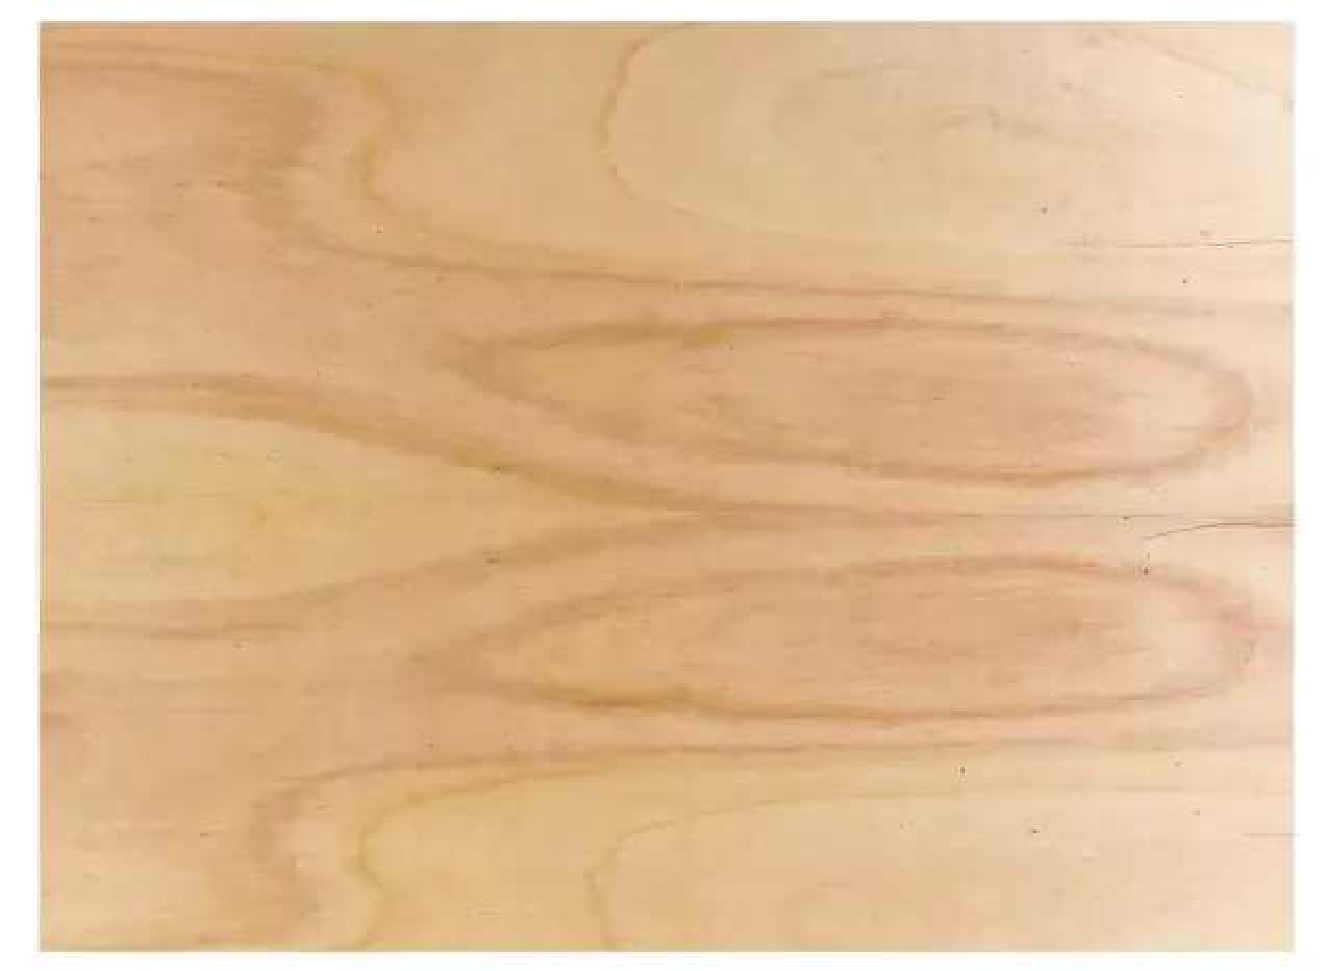
\includegraphics[width=0.6\textwidth]{Capitulos/3_hardware_softwares/3_figuras/compensado.pdf}}
	\caption*{Fonte: elaborado pelo autor (2023).}
	\label{fig3:image_02}
\end{figure}

\newpage
 Já para o braço do Aeropêndulo foi usando Tubo de Fibra de Vidro de Carbono 3x3x2mm, Figura \ref{fig3:image_03}, este material destaca-se por sua leveza e resistência física. No caso do braço do Aeropêndulo, localizado em sua extremidade, há um conjunto motor/hélice encarregado de impulsionar a dinâmica do sistema. Para otimizar o desempenho, é essencial minimizar a massa do braço. Ao fazer isso, as forças de resistência enfrentadas pela força de empuxo serão reduzidas, resultando em uma dinâmica mais ágil e eficiente do sistema.

\begin{figure}[!h]
	\centering
	\caption{Tubo de Fibra de Vidro de Carbono 3x3x2mm.}
	\efbox{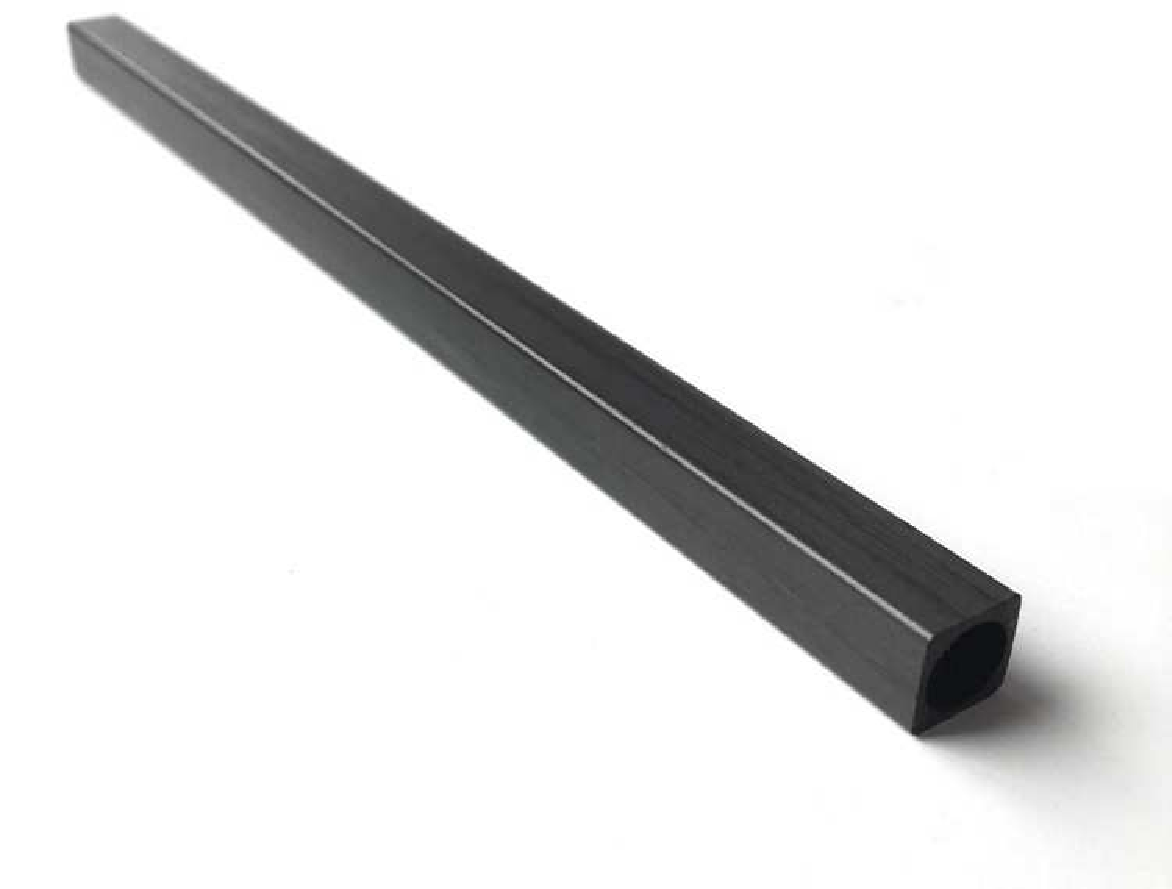
\includegraphics[width=0.5\textwidth]{Capitulos/3_hardware_softwares/3_figuras/carbono2x2mm.pdf}}
	\caption*{Fonte: elaborado pelo autor (2023).}
	\label{fig3:image_03}
\end{figure}


\subsection{Parte Elétrica do sistema}

Foram empregados os seguintes componentes eletrônicos no projeto: um Potenciômetro $50k\Omega$, uma Placa de desenvolvimento Esp32, um Módulo Driver L298n, um Conjunto (suporte/motor/hélice para drones fpv racing quadcopter) e componentes eletrônicos (resistor, capacitor).

\subsubsection{Potenciômetro $50k\Omega$}

O potenciômetro, Figura \ref{fig3:image_04}, desempenha o papel de \textit{encoder} ao obter o ângulo de inclinação do braço do Aeropêndulo. Essa funcionalidade é viabilizada pelo fato de que, conforme o braço se movimenta, a resistência do potenciômetro se altera, resultando em uma variação na tensão registrada em seus terminais. Essa interação permite estabelecer uma correlação entre a mudança na tensão elétrica e o ângulo de inclinação do braço do Aeropêndulo de maneira precisa e controlada.

\begin{figure}[!h]
	\centering
	\caption{Potenciômetro $50k\Omega$.}
	\efbox{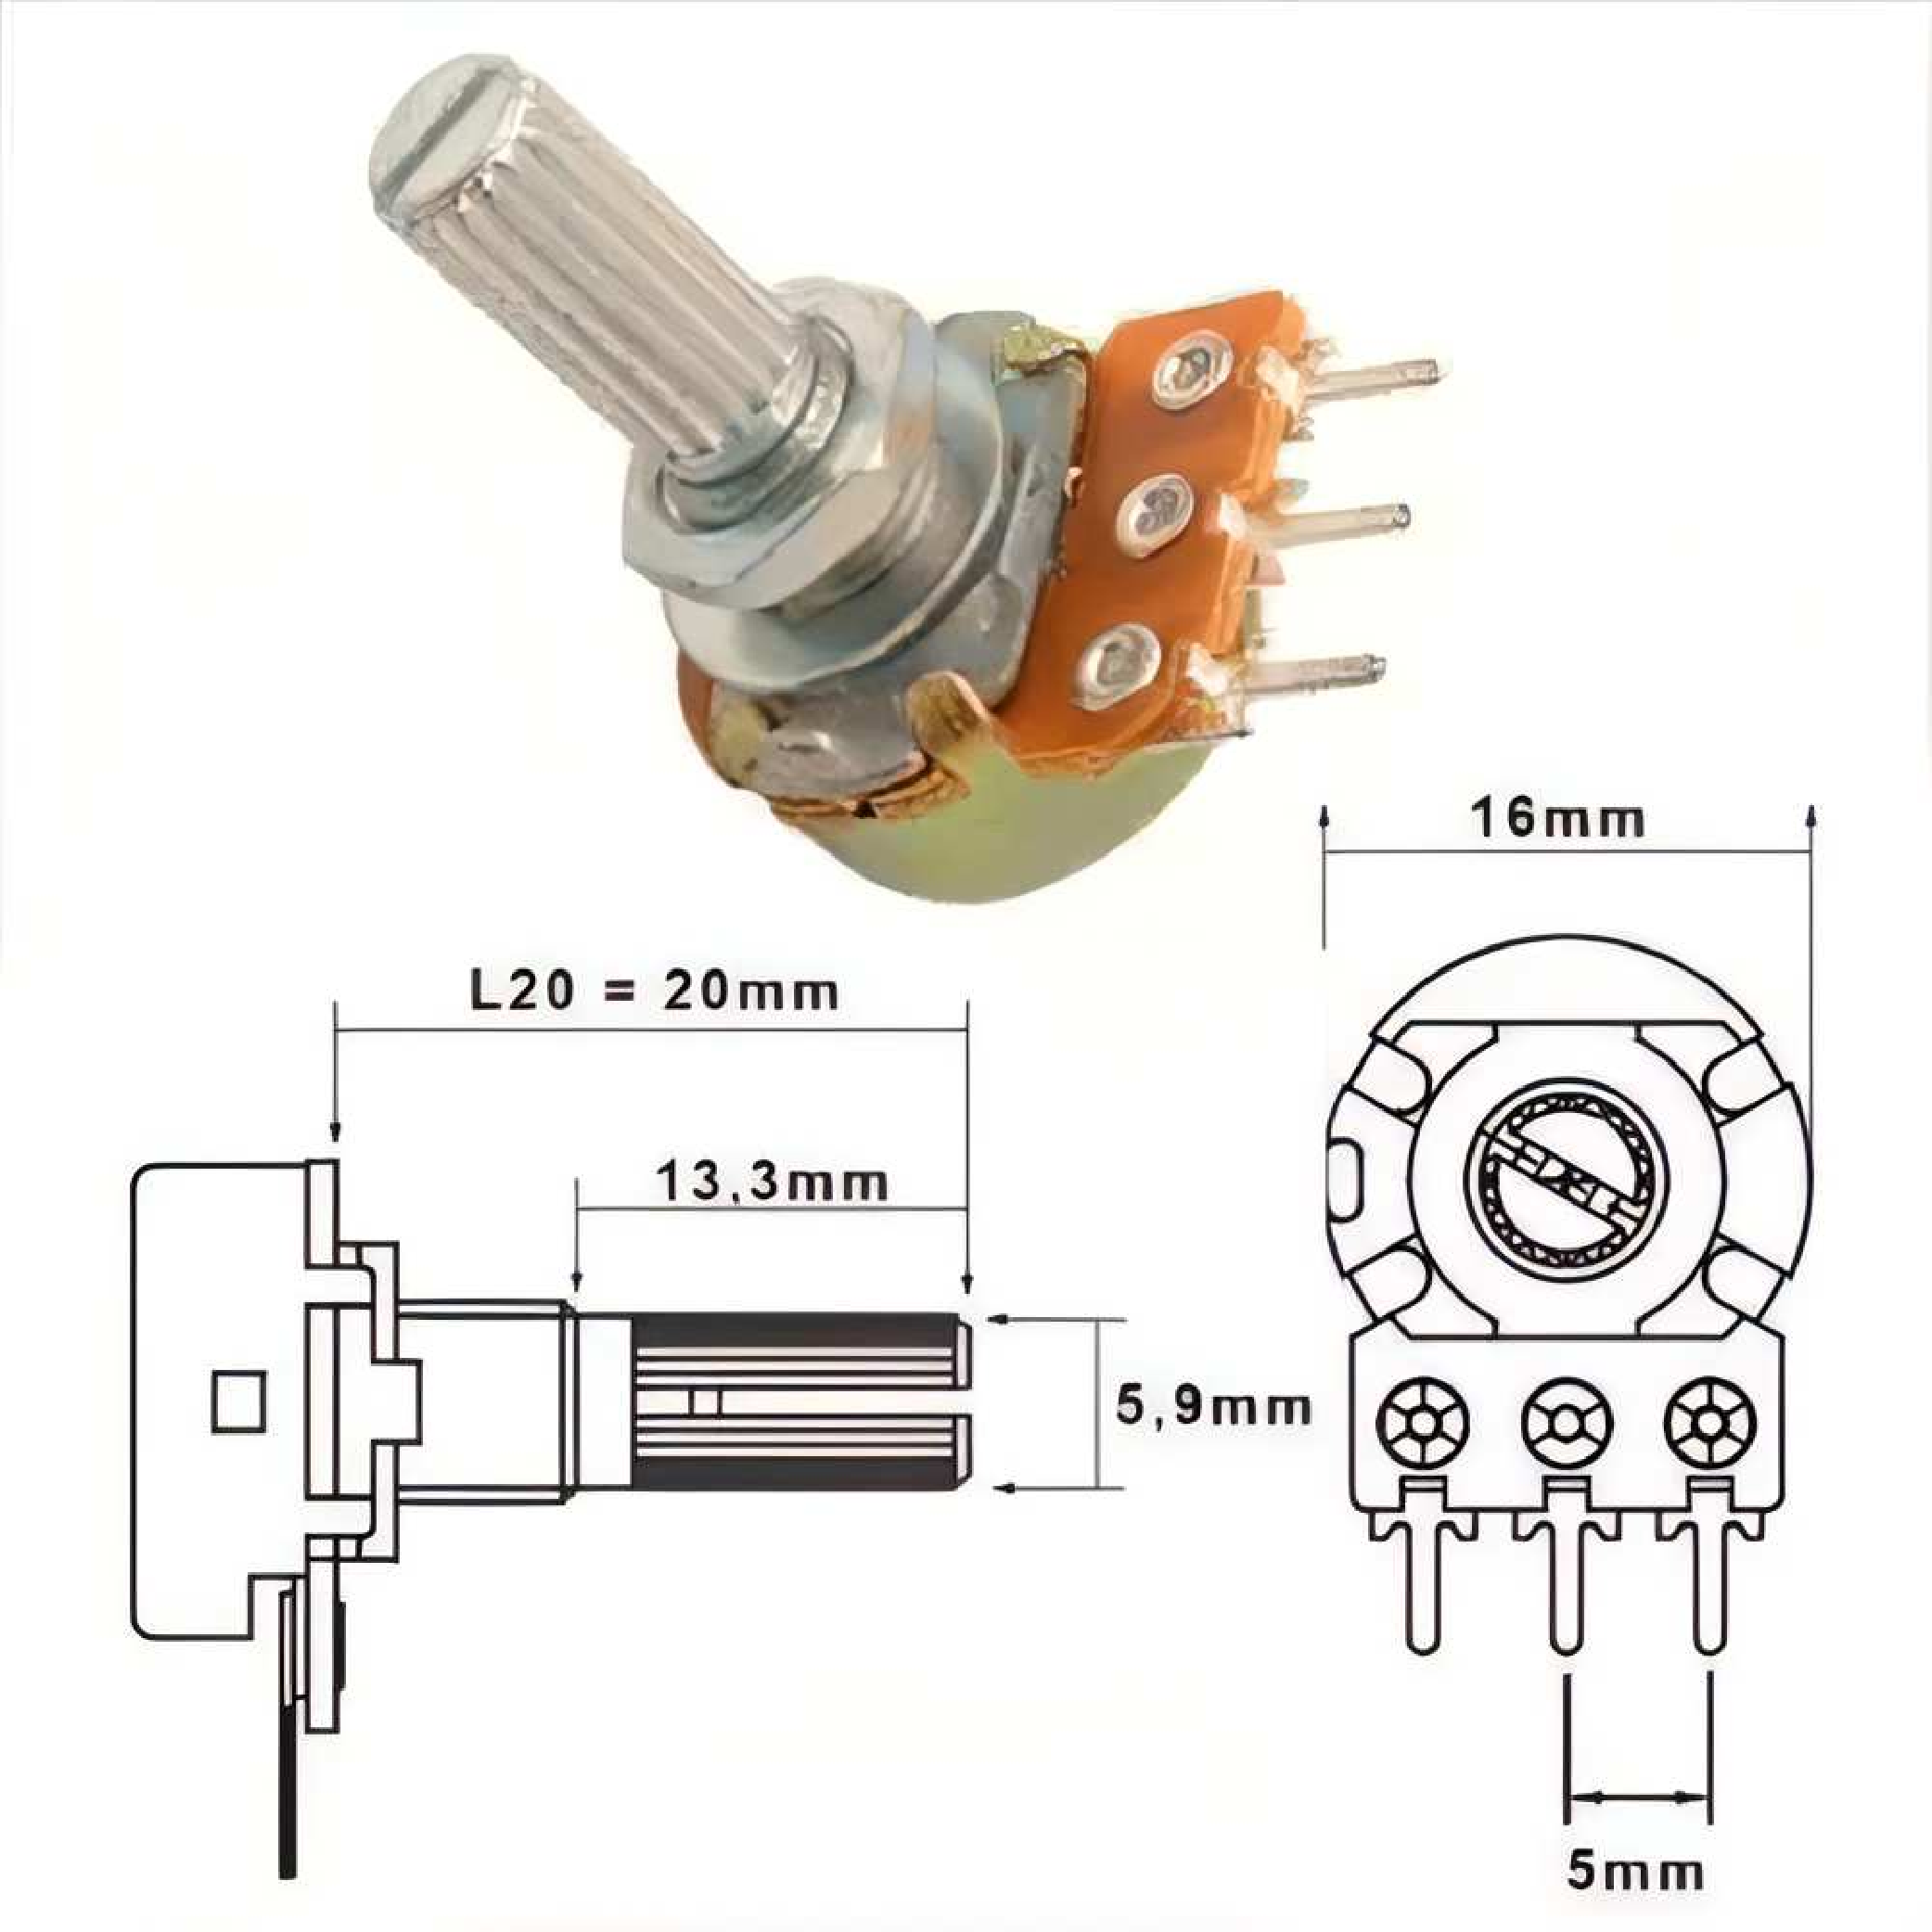
\includegraphics[width=0.5\textwidth]{Capitulos/3_hardware_softwares/3_figuras/pote.pdf}}
	\caption*{Fonte: elaborado pelo autor (2023).}
	\label{fig3:image_04}
\end{figure}




\subsubsection{Placa de desenvolvimento Esp32}

A placa de desenvolvimento ESP32 é uma poderosa e versátil plataforma que integra o popular microcontrolador ESP32 desenvolvido pela empresa  \textit{Espressif}. Projetada para atender às demandas de projetos de Internet das Coisas (IoT) e aplicações de conectividade sem fio, a ESP32 oferece uma vasta gama de recursos e funcionalidades. Equipada com um processador dual-core de 32 bits, Wi-Fi, Bluetooth, interfaces GPIO, I2C, SPI e UART, bem como suporte para memória externa.

A placa desempenhará uma função central no projeto, servindo tanto para a implementação do controlador discreto quanto para a obtenção de dados em tempo real relacionados aos estados do sistema. Esses estados incluem a leitura do sensor de ângulo do braço, a aquisição do sinal de controle e o cálculo do sinal de erro. Adicionalmente, a placa será empregada na geração dos sinais de referência necessários para o funcionamento ideal do sistema, A figura \ref{fig3:image_05} ilustra a placa de desenvolvimento Esp32.

\begin{figure}[!h]
	\centering
	\caption{Placa de desenvolvimento Esp32.}
	\efbox{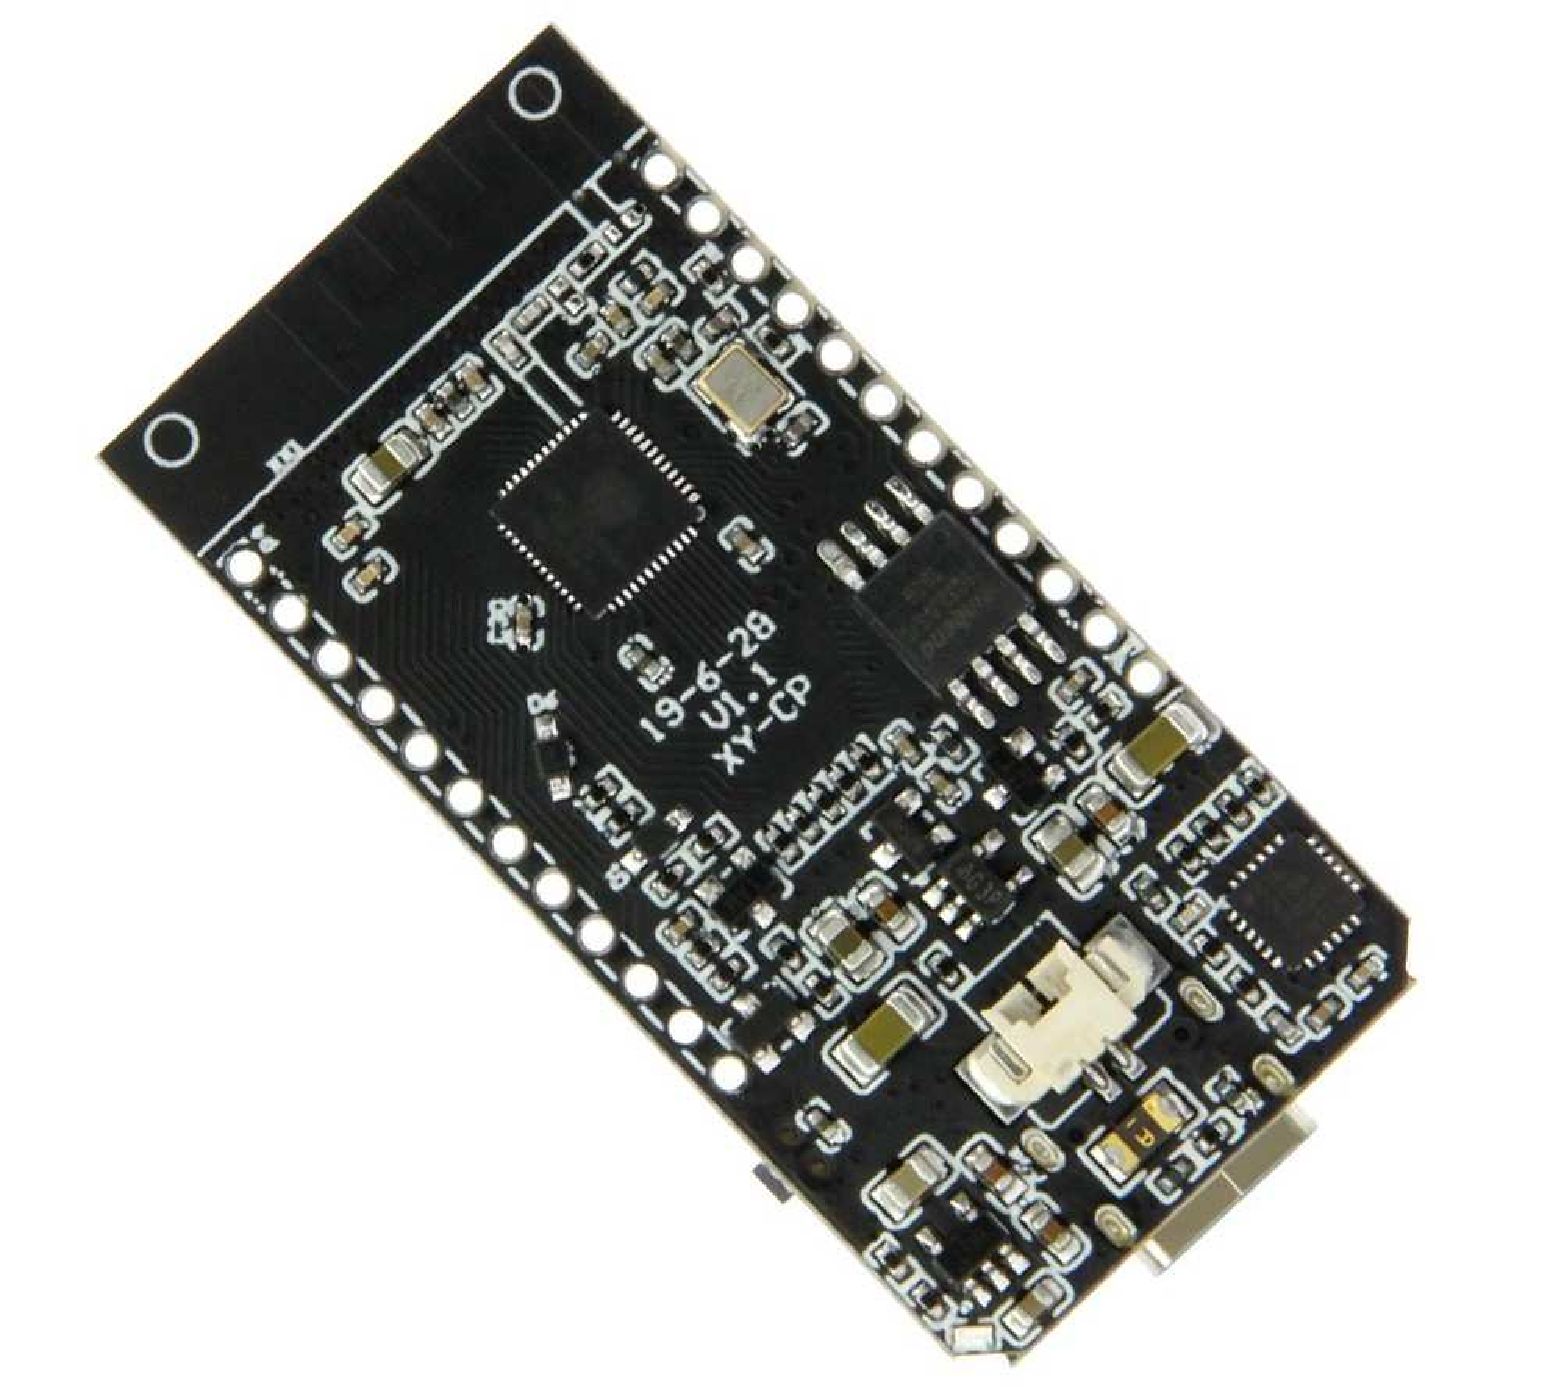
\includegraphics[width=0.5\textwidth]{Capitulos/3_hardware_softwares/3_figuras/f1_esp32.pdf}}
	\caption*{Fonte: elaborado pelo autor (2023).}
	\label{fig3:image_05}
\end{figure}


\subsubsection{Fonte Chaveada 2A, 5V, 25W}

Para a alimentação do motor CC série, foi usado uma fonte de alimentação de 5V/5A, Figura \ref{fig3:image_06}.

\begin{figure}[!h]
	\centering
	\caption{Fonte Chaveada 2A, 5V, 25W.}
	\efbox{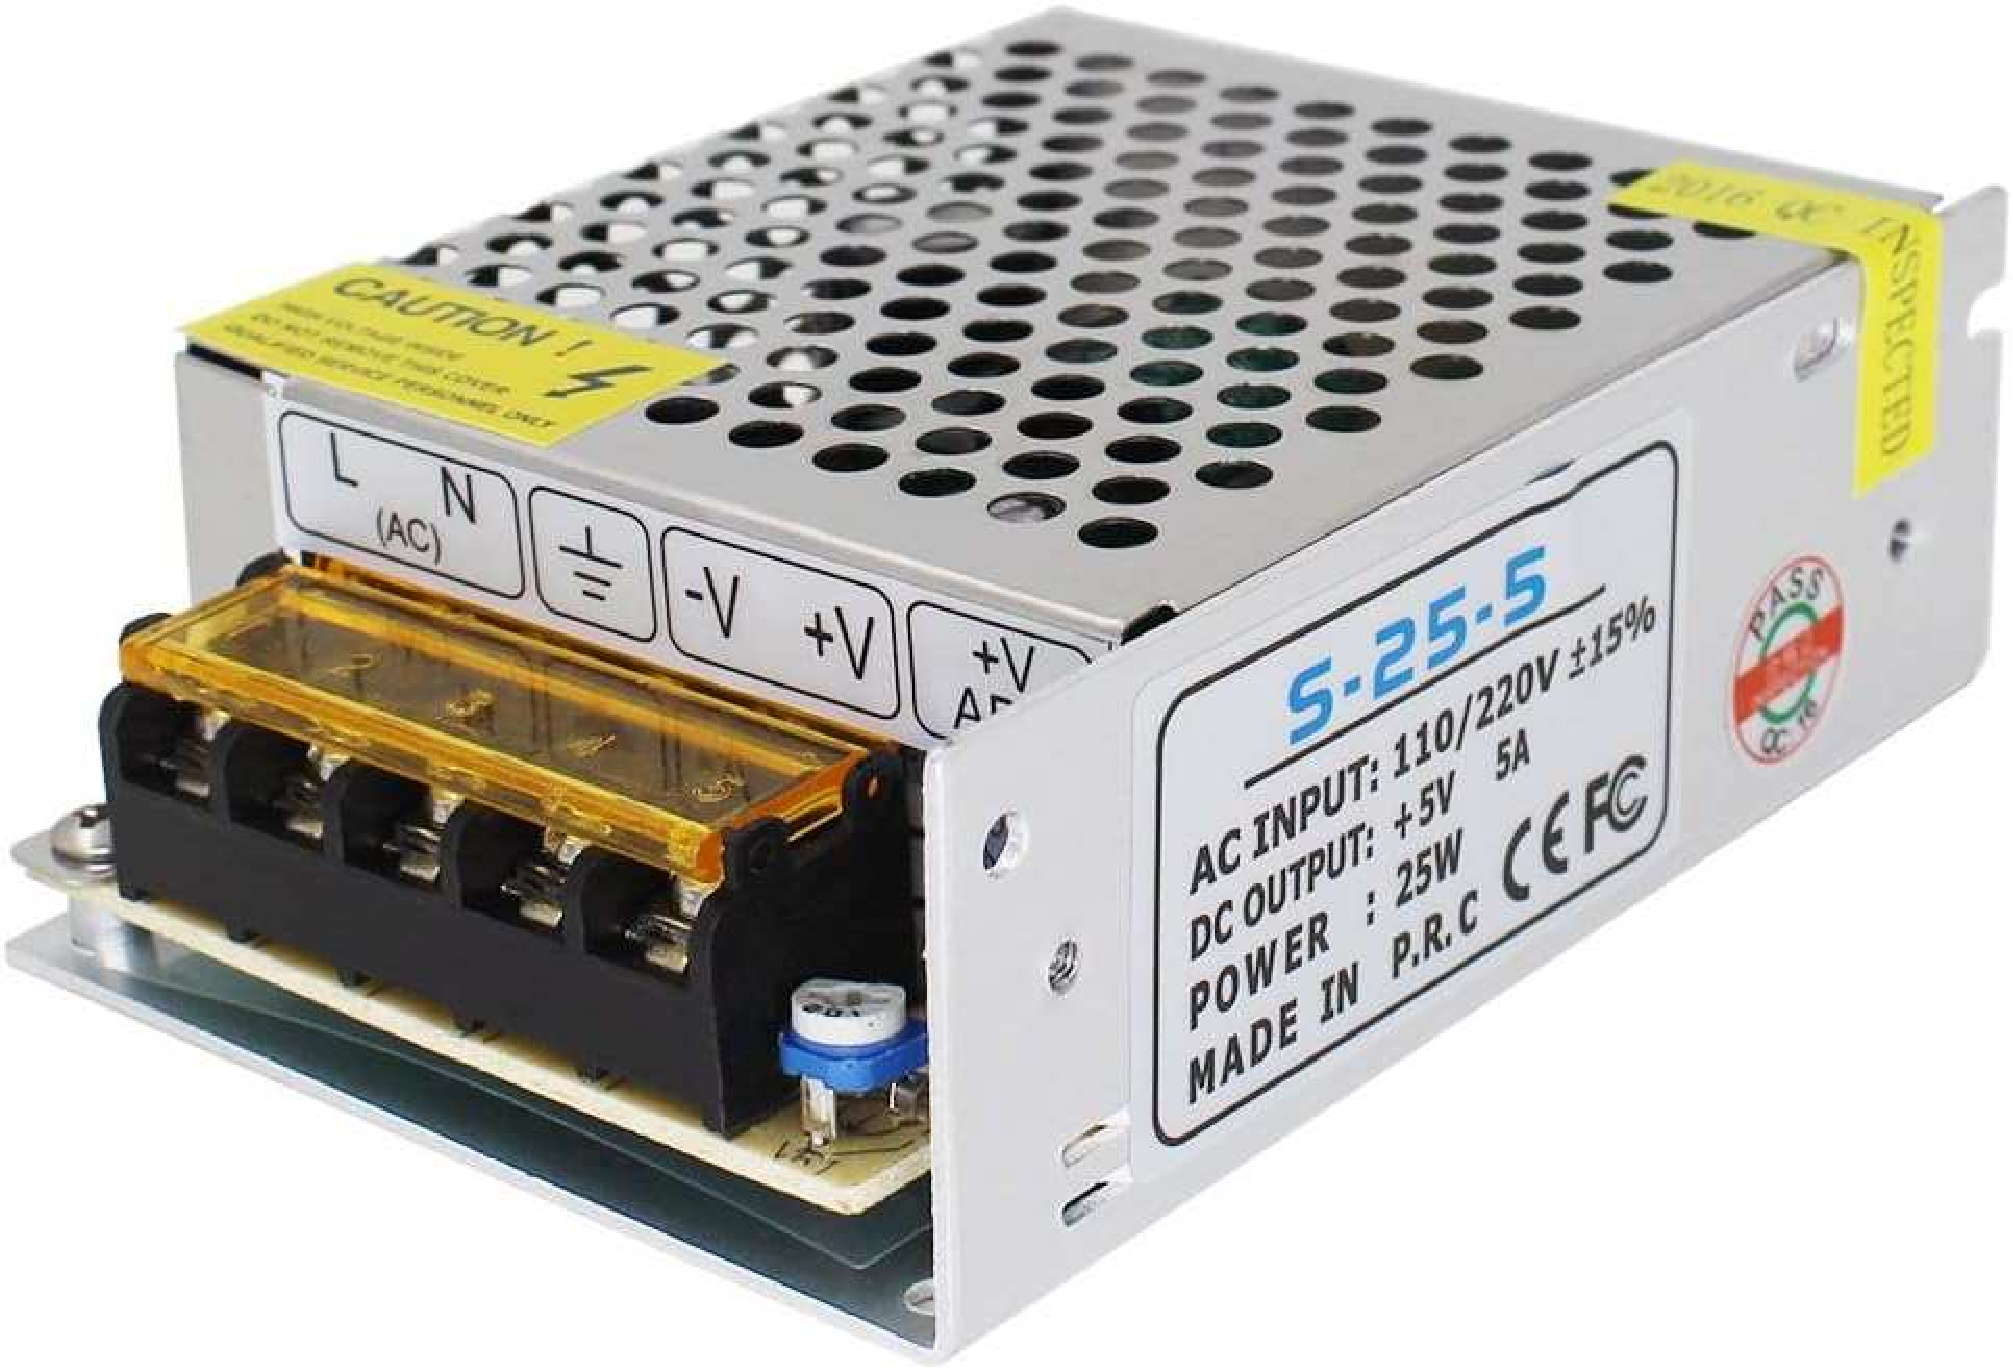
\includegraphics[width=0.45\textwidth]{Capitulos/3_hardware_softwares/3_figuras/f1_fonte.pdf}}
	\caption*{Fonte: elaborado pelo autor (2023).}
	\label{fig3:image_06}
\end{figure}



\subsubsection{Módulo Driver L298n}
\label{driver_l298n}

Para regular a velocidade no eixo do Motor CC série, empregou-se um Módulo Driver L298n, o qual possibilita controlar a injeção de potência entregue ao motor mediante a aplicação de um sinal PWM em sua entrada. Dessa forma, ao ajustar o sinal PWM, é possível obter uma tensão controlada aplicada de maneira precisa aos terminais do motor. A Figura \ref{fig3:image_07} ilustra o componente em questão.

\begin{figure}[!h]
	\centering
	\caption{Módulo Driver L298n.}
	\efbox{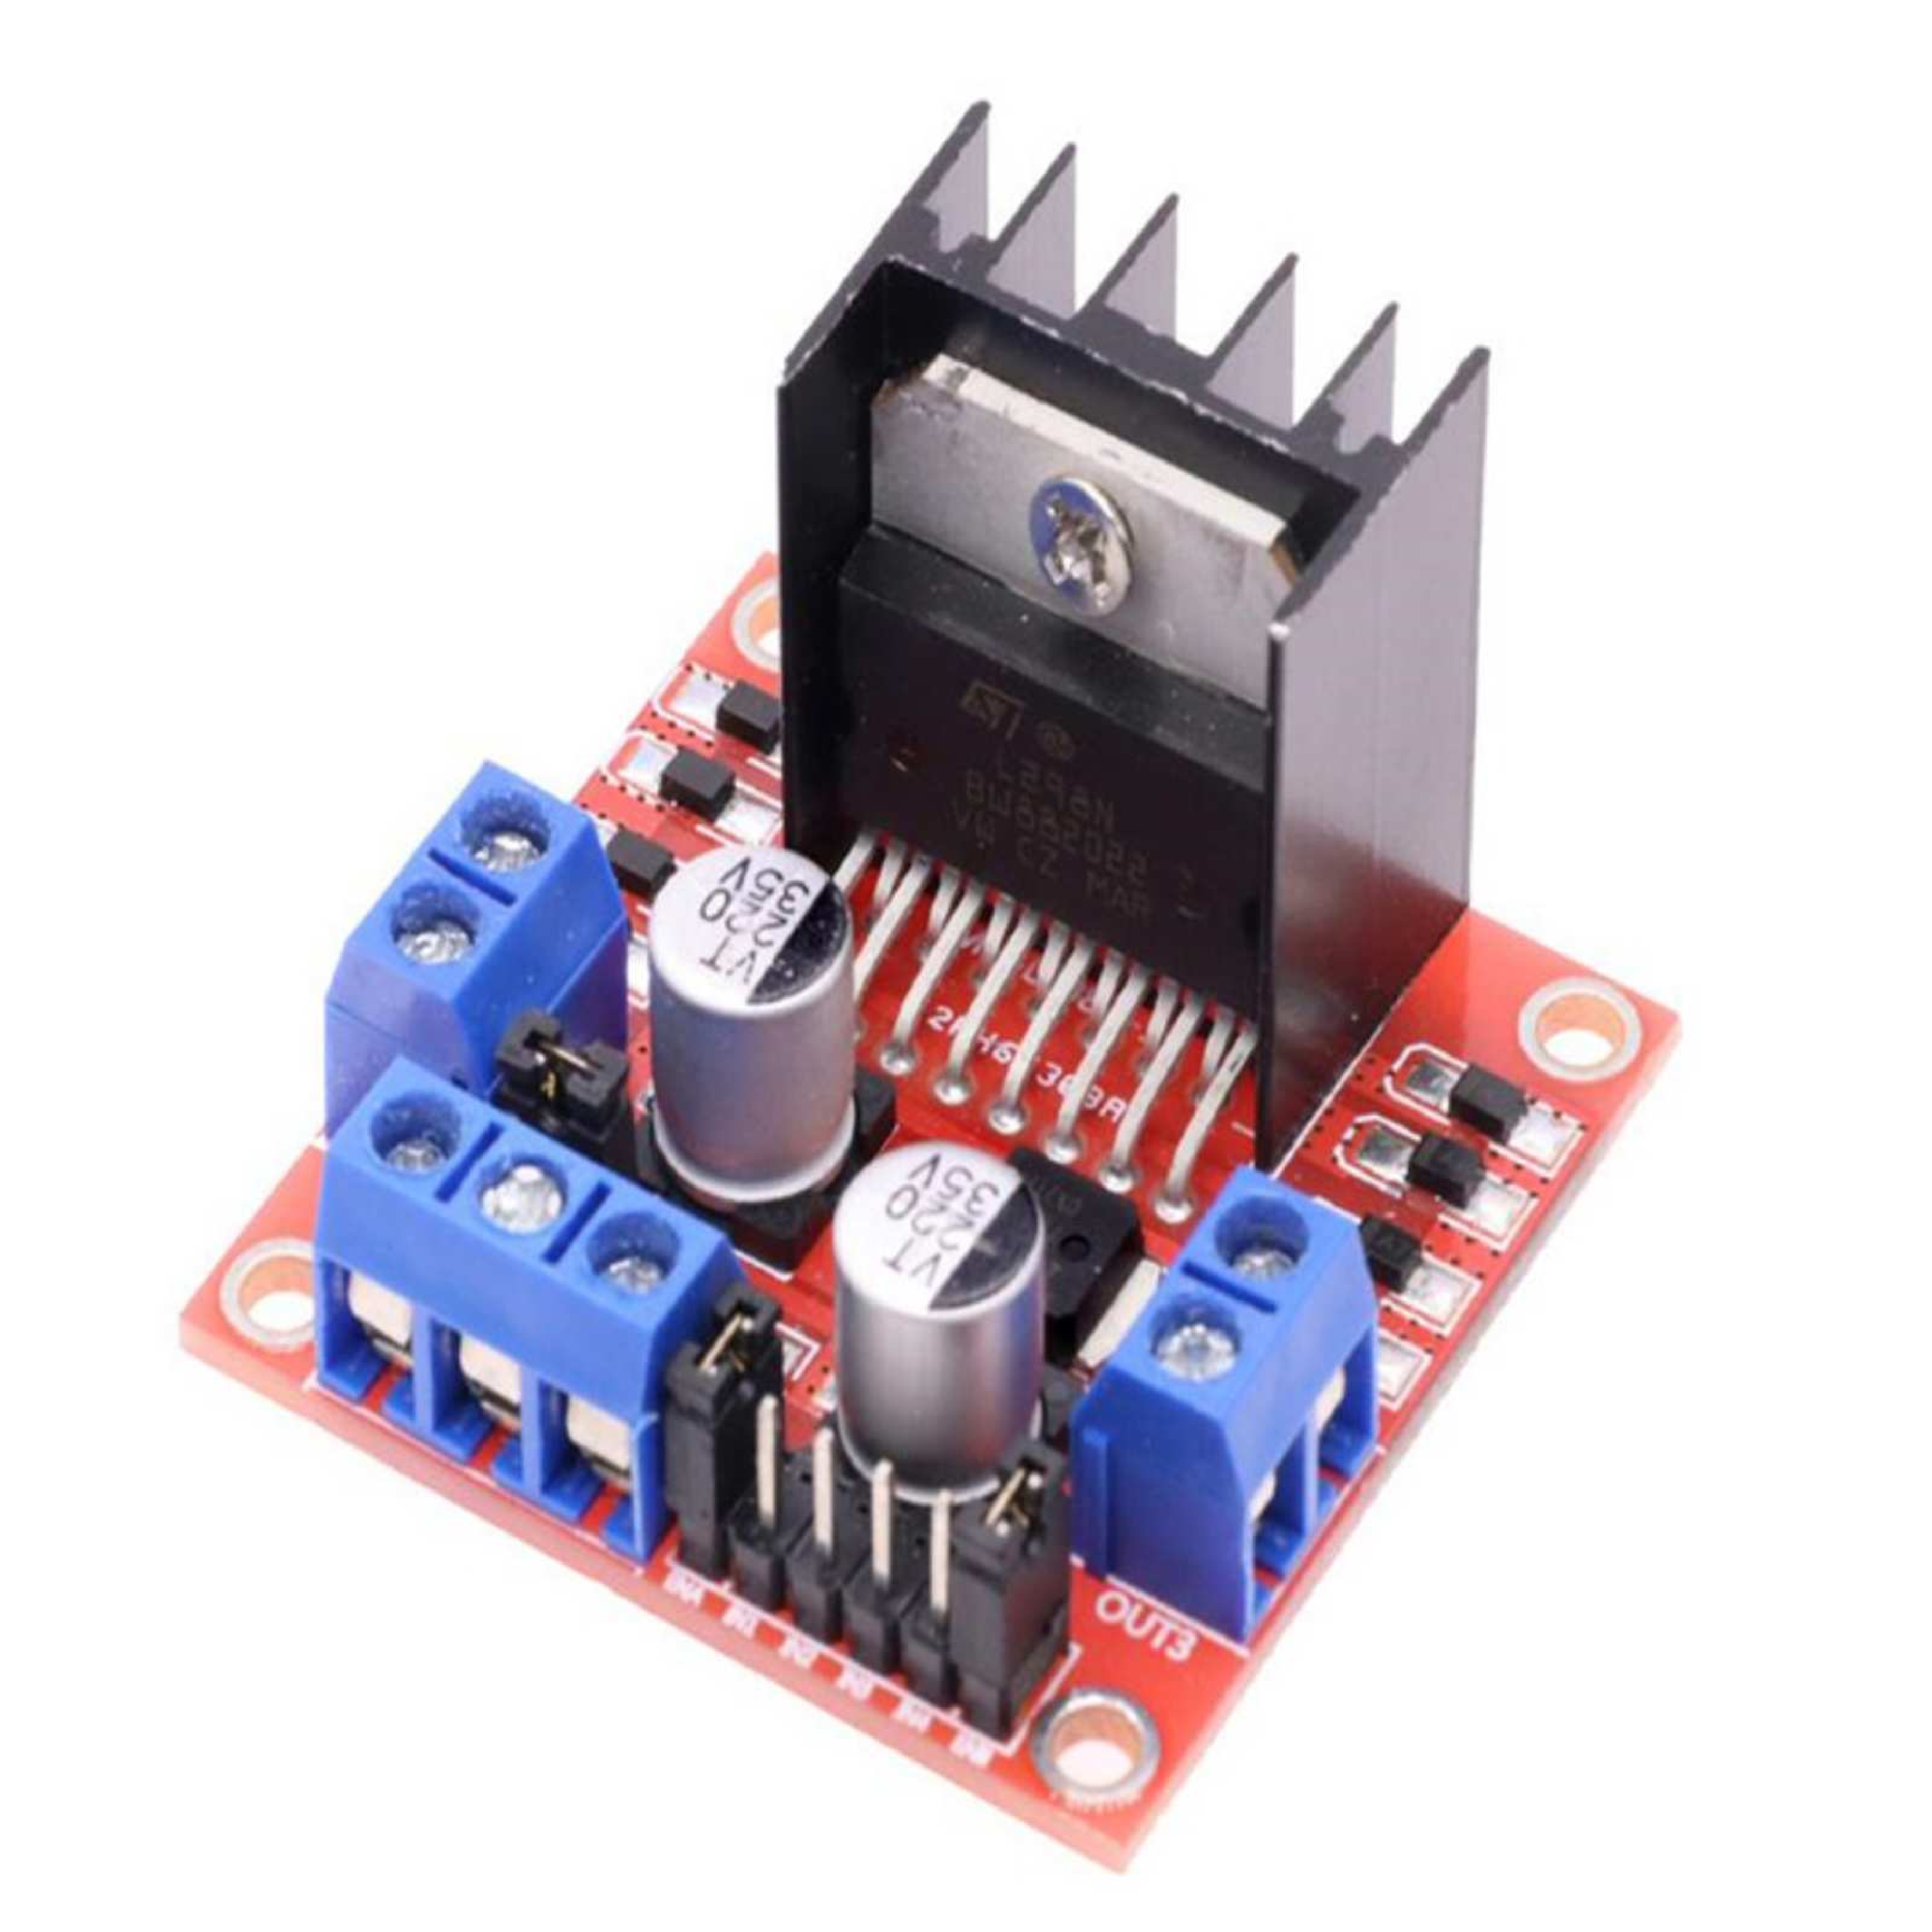
\includegraphics[width=0.45\textwidth]{Capitulos/3_hardware_softwares/3_figuras/f4_ponteH.pdf}}
	\caption*{Fonte: elaborado pelo autor (2023).}
	\label{fig3:image_07}
\end{figure}


\subsubsection{Conjunto (suporte motor cw/ccw hélice) para drones fpv racing quadcopter}


A obtenção da força de empuxo na extremidade do braço do Aeropêndulo foi realizada por meio de um conjunto composto por suporte, motor e hélice projetado originalmente para drones FPV Racing Quadcopter. Esse conjunto demonstrou ser ideal para aplicação no Aeropêndulo devido à sua eficiência e desempenho em ambientes dinâmicos. A Figura \ref{fig3:image_08} fornece uma representação visual esclarecedora desse componente crucial, destacando sua integração perfeita no contexto do experimento.


\begin{figure}[!h]
	\centering
	\caption{Conjunto (suporte motor cw/ccw hélice).}
	\efbox{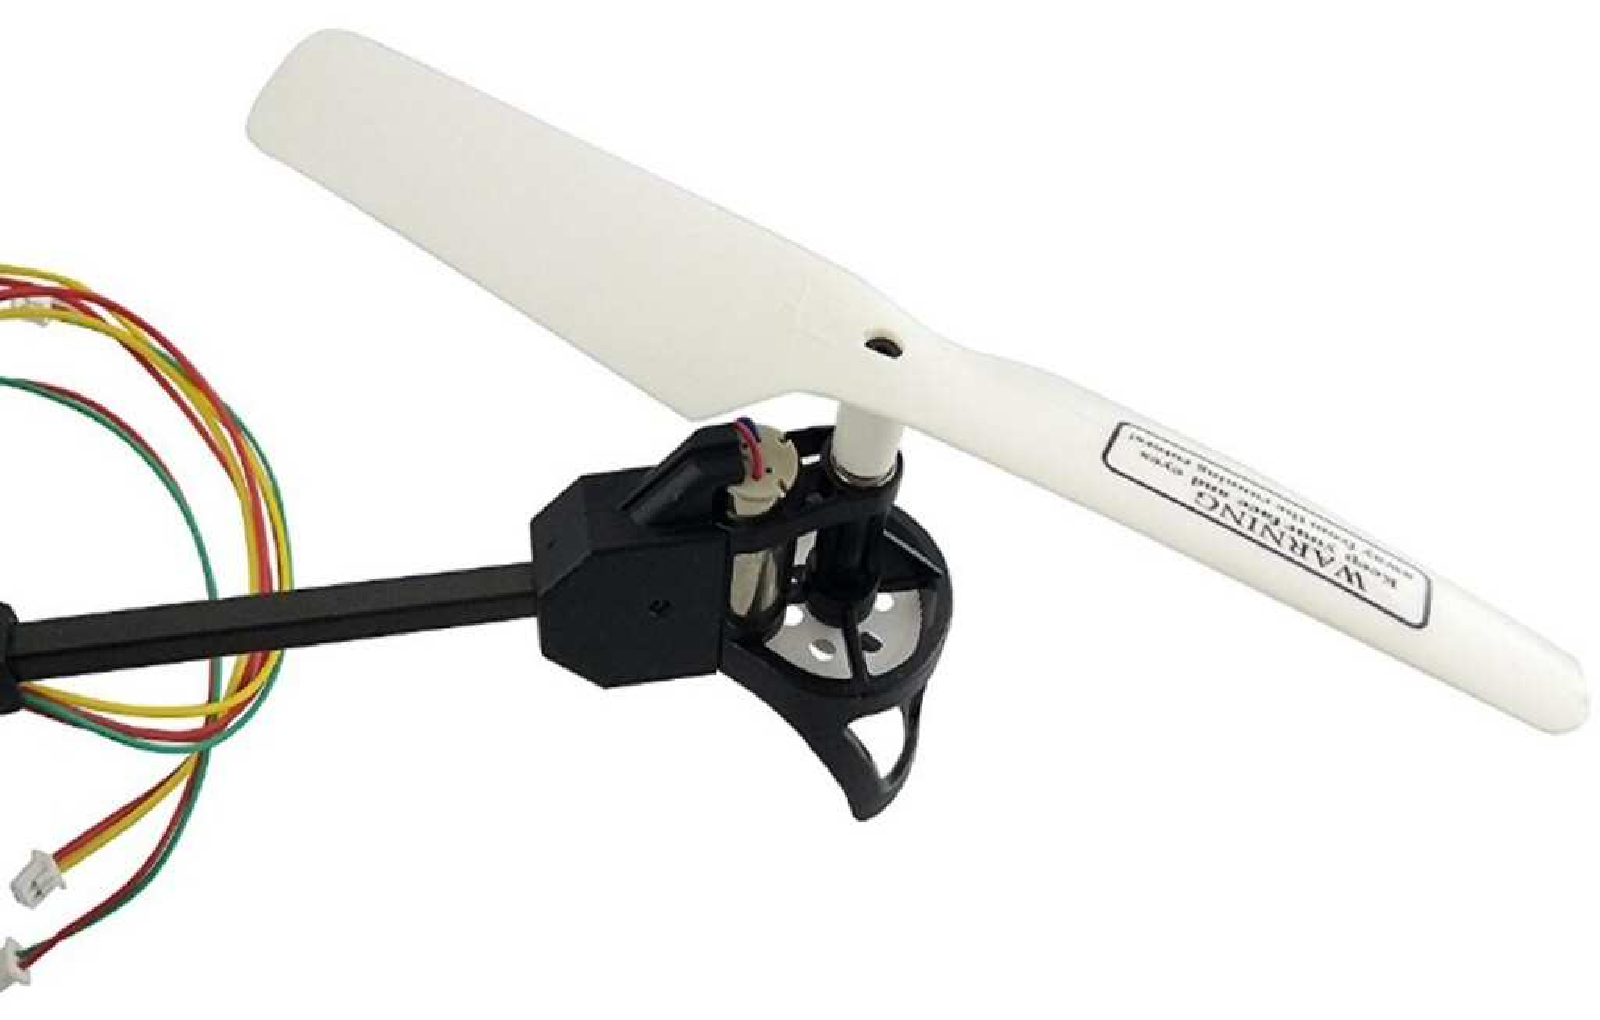
\includegraphics[width=0.5\textwidth]{Capitulos/3_hardware_softwares/3_figuras/f1_braco_aerop.pdf}}
	\caption*{Fonte: elaborado pelo autor (2023).}
	\label{fig3:image_08}
\end{figure}

\newpage
\subsubsection{Componentes eletrônicos (resistivos e capacitivos)}

Por fim, para que o sinal do sensor (Potenciômetro) seja de boa qualidade, foi usado um filtro RC série, dessa forma, empregou-se um capacitor de um resistor na implementar do filtro. A Figura \ref{fig3:image_09} corresponde aos componentes resistivos e a Figura \ref{fig3:image_10} aos componentes capacitivos.


\begin{figure}[!h]
         \centering
         \caption{Resistores.}
         \efbox{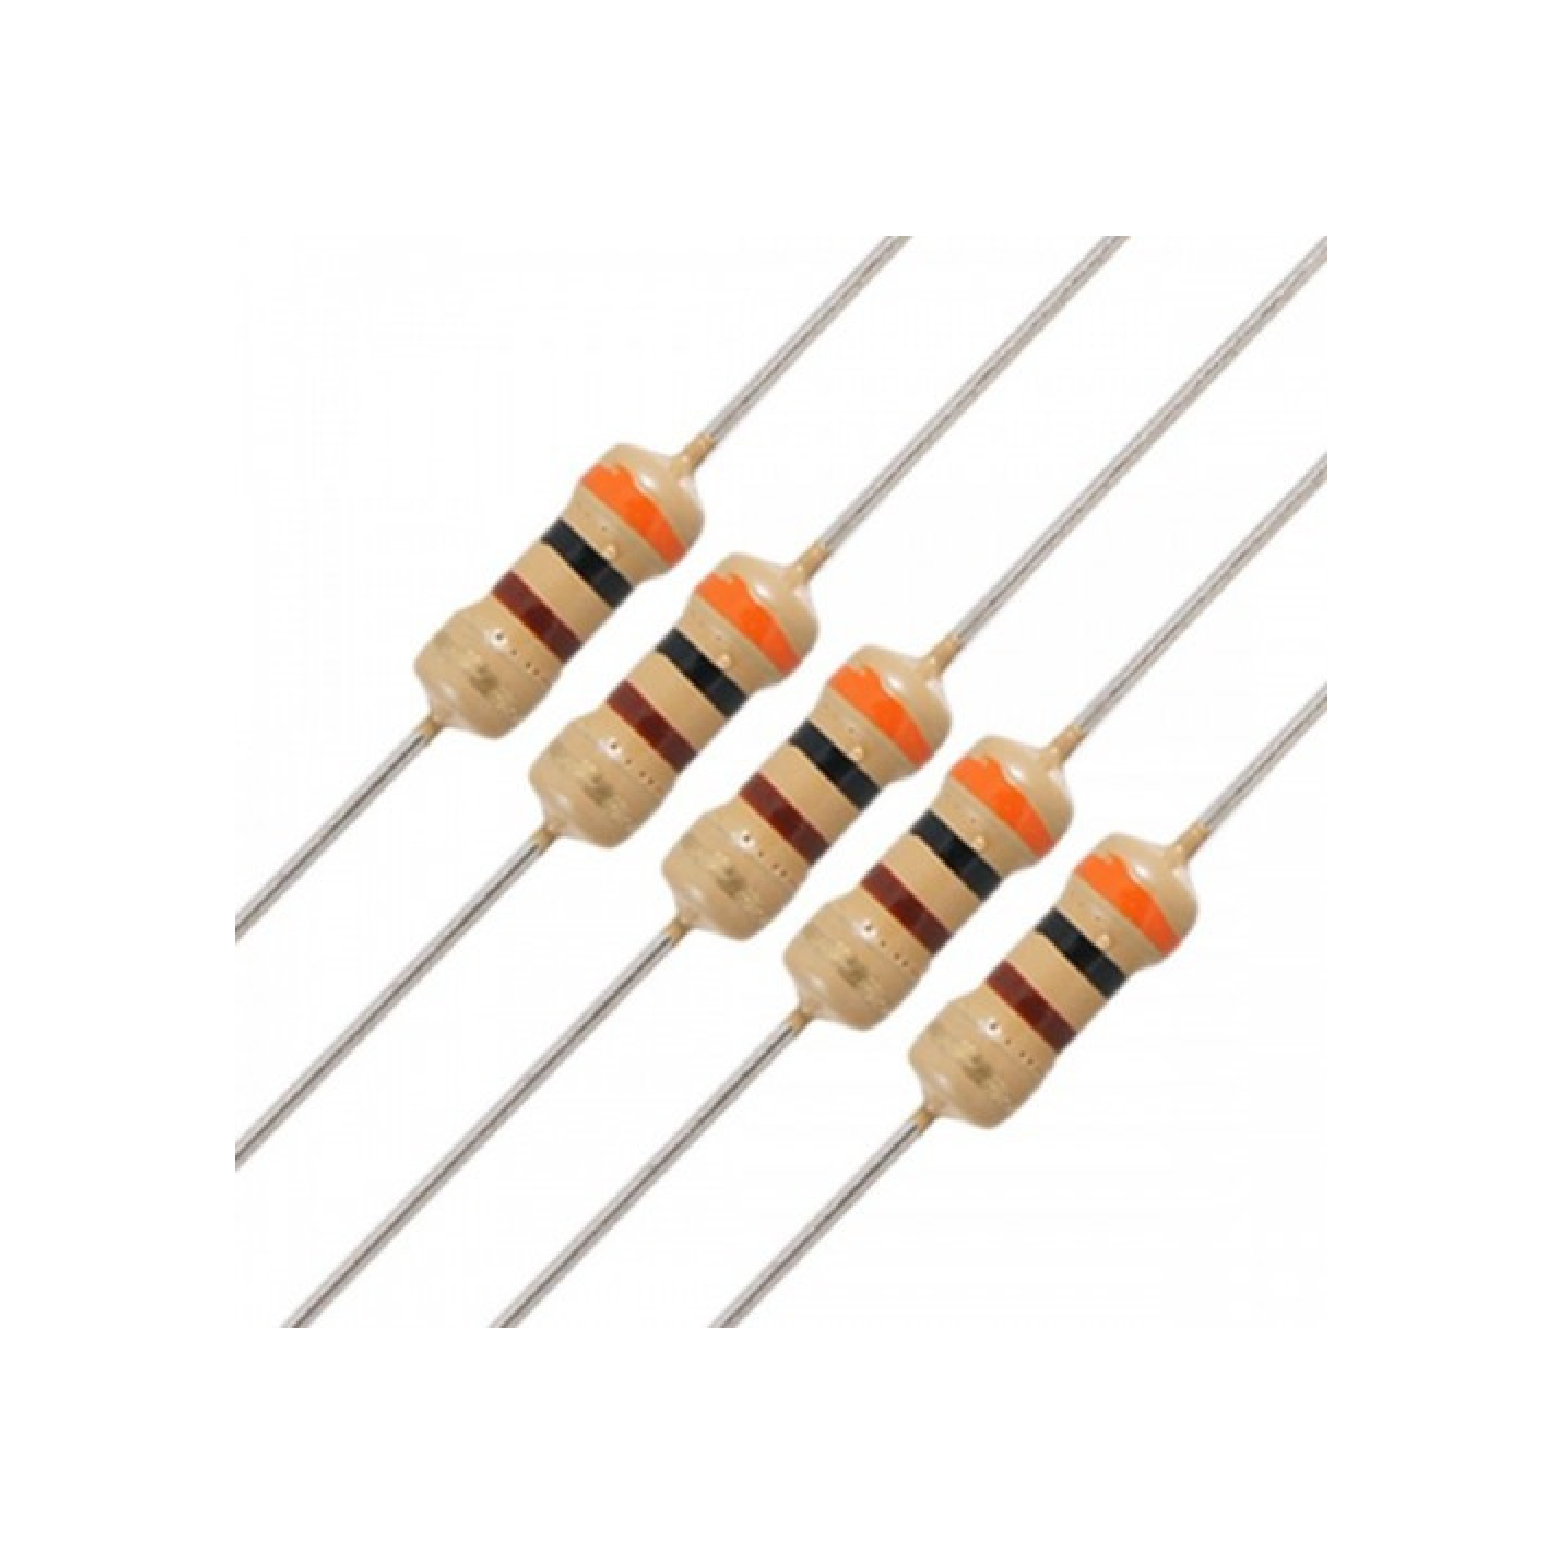
\includegraphics[width=0.5\textwidth, page=1]{Capitulos/3_hardware_softwares/3_figuras/res_cap.pdf}}
         \caption*{Fonte: elaborado pelo autor (2023).}
         \label{fig3:image_09}
\end{figure}

\begin{figure}[!h]
         \centering
         \caption{Capacitores.}
         \efbox{\includegraphics[width=0.5\textwidth, page=2]{Capitulos/3_hardware_softwares/3_figuras/res_cap.pdf}}
         \caption*{Fonte: elaborado pelo autor (2023).}
         \label{fig3:image_10}
\end{figure}


\subsection{Montagem do Protótipo}

\subsubsection{Parte Física}

O protótipo foi concebido visando a desmontagem da estrutura, permitindo um transporte mais conveniente. A construção física compreende três componentes com pontos de conexão estratégicos. Ademais, o braço do Aeropêndulo pode ser facilmente desacoplado no ponto de pivô, onde se conecta ao eixo do potenciômetro.

Para montar a estrutura, basta acoplar suas partes. Com isso, a componente estrutural estará pronta para uso. O resultado final do sistema ficou notavelmente estável, com a estrutura demonstrando rigidez suficiente para evitar vibrações indesejadas no braço do Aeropêndulo durante o acionamento.

\subsubsection{Parte Elétrica}


A Figura \ref{fig3:image_11} ilustra a dinâmica do fluxo de interligação do sistema elétrico do Aeropêndulo. Notavelmente, o microcontrolador desempenha um papel central ao gerar o sinal de controle PWM, realiza a leitura do sinal filtrado proveniente do sensor (Potenciômetro) e estabelecer comunicação com o computador através da interface serial. Adicionalmente, o driver é alimentado por uma fonte de tensão contínua de 5V, o qual amplifica e aplica o sinal de controle ao motor CC Série. Esta ação, por sua vez, resulta em uma variação angular no braço do Aeropêndulo por conta do empuxo gerado pelas hélices, impactando diretamente o estado do sensor (Potenciômetro) e sua saída correspondente.

\begin{figure}[!h]
	\centering
	\caption{Diagrama de comunicação do Aeropêndulo.}
	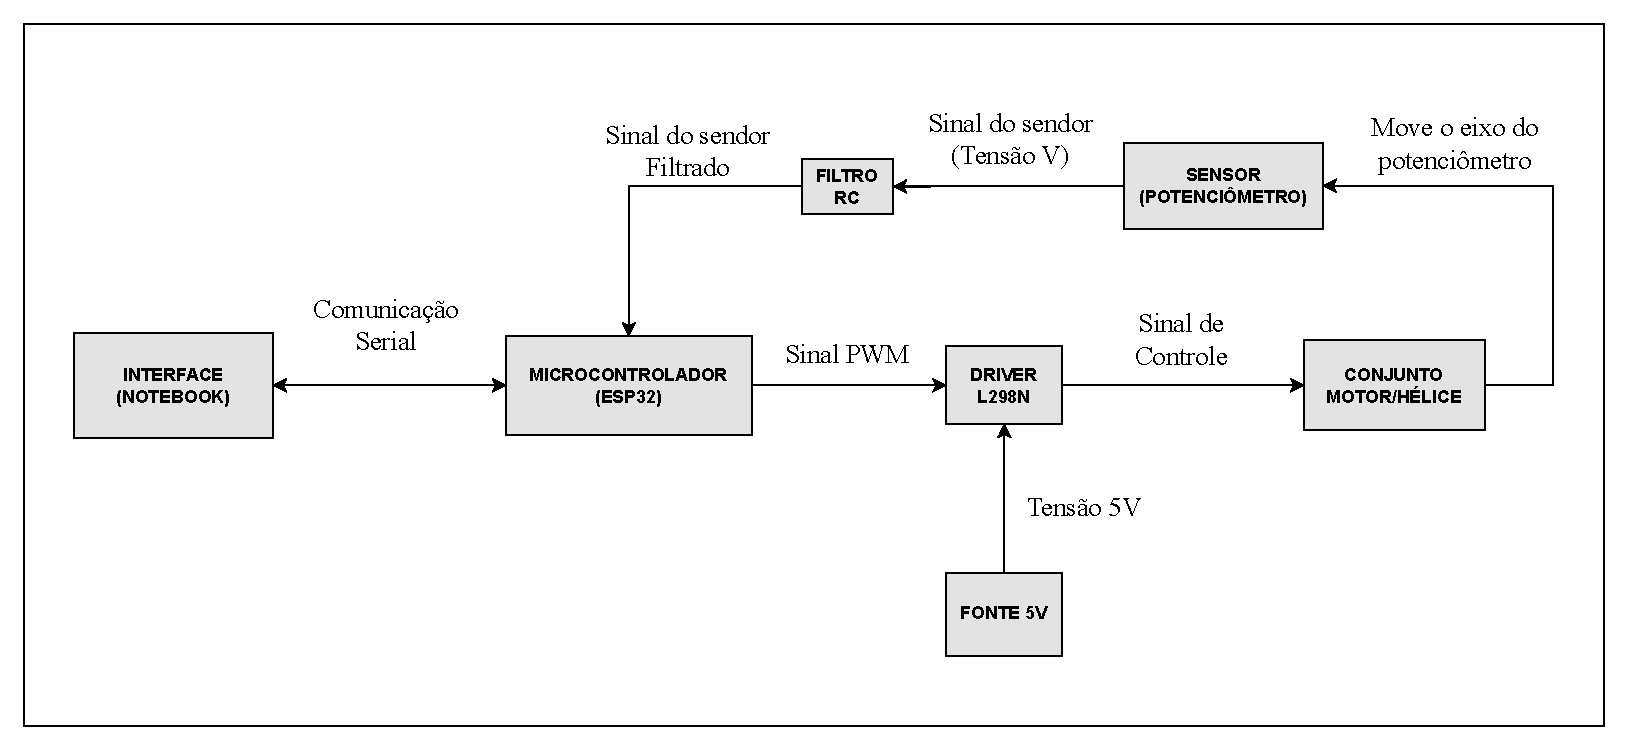
\includegraphics[width=0.9\textwidth, page=1]{Capitulos/3_hardware_softwares/3_figuras/diag_aerop.pdf}
	\caption*{Fonte: elaborado pelo autor (2023).}
	\label{fig3:image_11}
\end{figure}



O esquema de ligação dos componentes do sistema elétrico é exemplificado na Figura \ref{fig3:image_12}.

\begin{figure}[!h]
	\centering
    	\caption{Esquema de conexões elétricas do Aeropêndulo.}
	\efbox{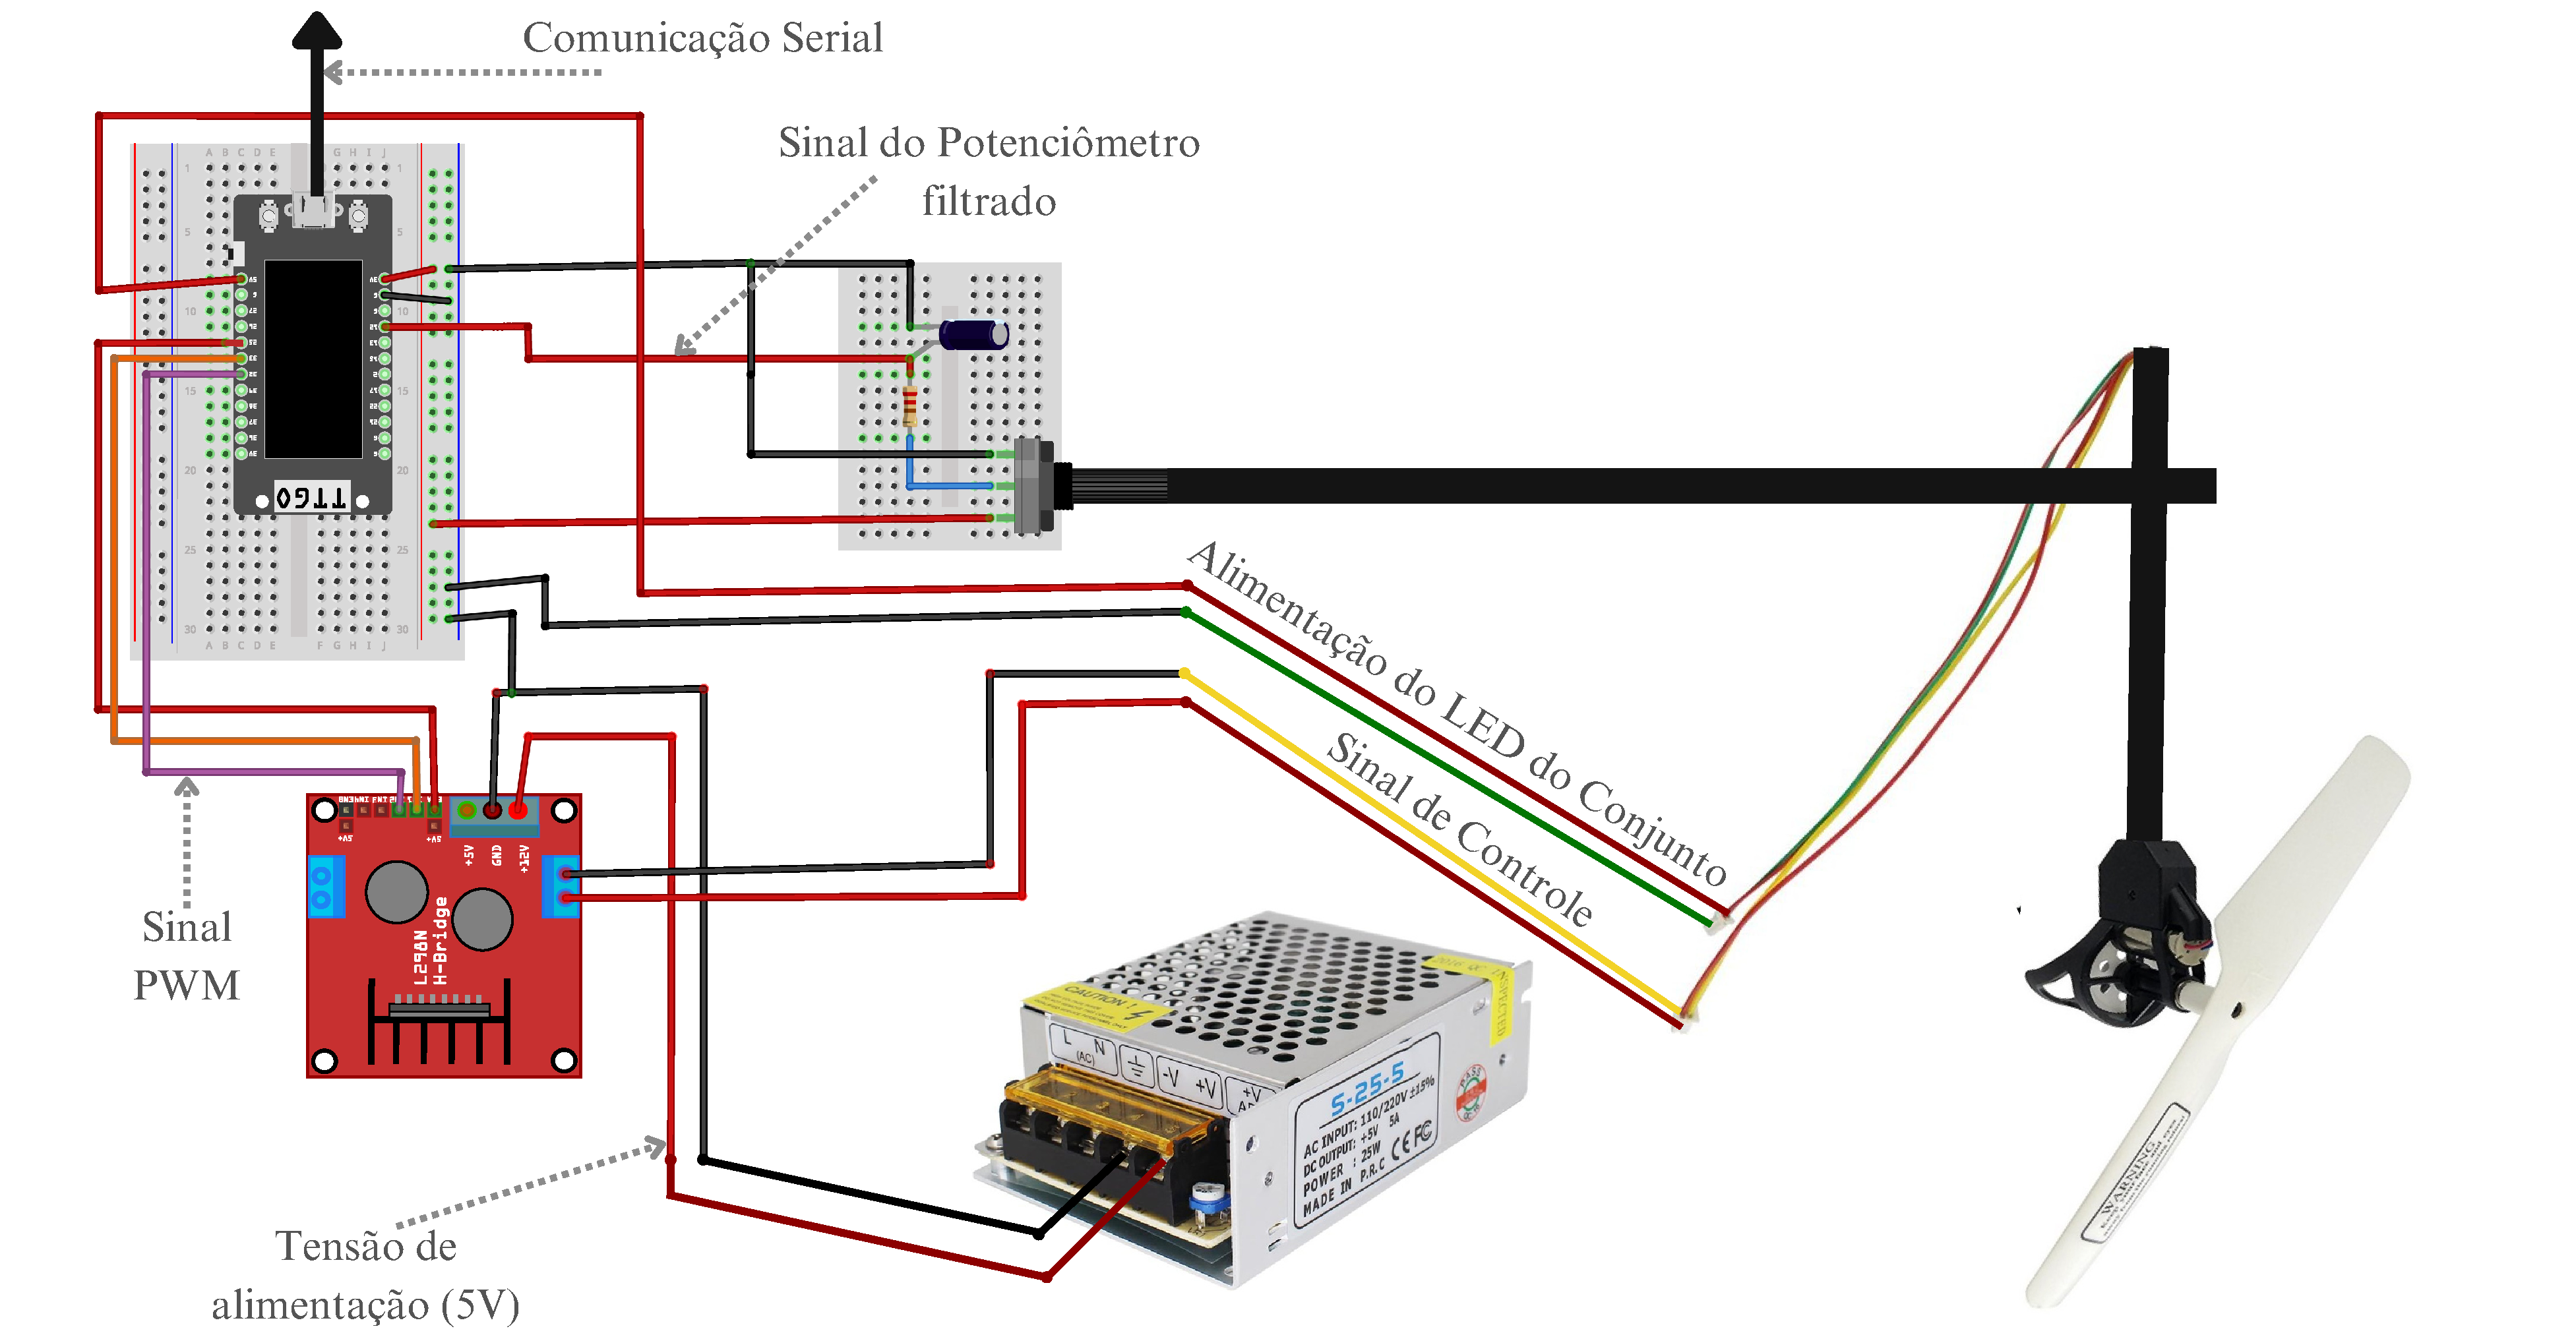
\includegraphics[width=1\textwidth, page=1]{Capitulos/3_hardware_softwares/3_figuras/esquema_eletrico_aerop.pdf}}
	\caption*{Fonte: elaborado pelo autor (2023).}
	\label{fig3:image_12}
\end{figure}

\vspace{2cm}
